\section{Статья 1: Исследование способов кодирования и создания синтаксических деревьев в программировании с экспрессией генов}

\subsection{Введение}

Эволюционные вычисления~--- термин, применяемый к техникам глобальной оптимизации, характерной особенностью которых является подобие их процессов биологической эволюции. Вместо работы с одним определённым вариантом решения, эволюционные техники начинают процесс поиска с популяции вариантов решения, созданных случайным образом. Начальная популяция эволюционирует в набор улучшенных решений, итеративно проходя три этапа: отбор, рекомбинация и мутация. Наиболее приспособленные решения отбираются для участия в рекомбинации для создания нового поколения, а оператор мутации вносит в него разнообразие. В ходе этого процесса лучшие особи передают свои характеристики следующим поколениям. При достаточном количестве итераций эволюционные алгоритмы способны находить решения многих сложных задач.

Функция, определяющая количественную оценку особи~--- степень соответствия построенной модели условию задачи~--- называется функцией фитнеса (fitness function), чаще всего применяется значение среднеквадратичного отклонения (СКО). При таком подходе генетическое программирование и другие эволюционные техники могут за короткое время находить оптимальные либо около-оптимальные решения задач и ситуаций. Используя эти техники, не требуется индивидуальный ручной поиск оптимального решения каждой задачи~--- описанный процесс автоматизирован и выполняется компьютером, однако для этого требуются значительные вычислительные ресурсы~\cite{Nunez:2006:msoec}.

Генетические алгоритмы (ГА) были созданы в 1960-е, когда Джон Холланд применил теорию биологической эволюции к компьютерным системам~\cite{Holland:1975}. Как и все эволюционные компьютерные системы, ГА представляет собой упрощённую модель билогической эволюции. При таком подходе варианты решения задач кодируются символьными строками (обычно состоящими из нулей и единиц), и популяция этих вариантов решения участвует в процессе эволюции, цель которой~--- получение наилучшего решения.

Развитие идеи кодирования нелинейных структур разных размеров и форм Джоном К\'{о}зой привело к появлению в 1992 году генетического программирования (ГП)~\cite{Koza92}.

Программирование с экспрессией генов (ПЭГ), как в целом и ГА и ГП, является генетическим алгоритмом с такими характерными чертами как популяция особей, их отбор на основе приспособленности (фитнеса), изменчивость на основе генетических операторов~\cite{Ferreira2001}. Фундаментальное отличие этих трёх алгоритмов заключается в природе особей: в ГА это строки фиксированной длины (хромосомы); в ГП~--- нелинейные сущности переменной длины и формы (синтаксические деревья). В ПЭГ особи кодируются в виде строк фиксированной длины (называемых геномом, либо хромосомами~\cite{ferreira:2001:wsc6Aa}), которые затем декодируются для получения синтаксических деревьев.

Различие между ГА и ГП выражено не сильно: обе системы используют один вид объектов, который служит как генотипом, так и фенотипом. Такой подход имеет одно из двух ограничений: простота применения генетических операторов к объектам означает их недостаточную выразительность и сложность этих объектов (в случае ГА), а их сложность ведёт к трудностям при воспроизводстве и модификации (в случае ГП).

ПЭГ лишено указанных ограничений и обладает следующими преимуществами:
\begin{itemize}
  \item Простота хромосом: линейность, компактность, относительно небольшой размер, простота применения операторов, таких как репликация, мутация, рекомбинация, перенос и пр.
  \item Экспрессия (декодирование компактной структуры) генома порождает фенотип~--- синтаксическое дерево, которое может представлять математическую формулу либо программу. Значения вычисленной формулы, выполненной программы служат для численной оценки приспособленности особи с помощью функции фитнеса.
\end{itemize}

Таким образом, участие хромосомы в процессе воспроизведения зависит от фитнеса дерева, которое она кодирует. Для этого требуется универсальная система перевода формата генома в формат дерева и обратно, при которой любое изменение хромосомы с помощью операторов всегда приводит к синтаксически корректному дереву, обеспечивая приспосабливаемость и эволюционирование.



%--------------------------------------------------------------------



\subsection{Исходный алгоритм ПЭГ}

На рисунке~\ref{img:GEP_flowchart} показана блок-схема алгоритма ПЭГ~\cite{Ferreira2001}.

\begin{figure} [h]
\center
\begin{tikzpicture}[node distance = 5mm, every node/.style={transform shape}]
  \node [block] (create) {Создание начальной популяции};
  \node [block,    below = of create]   (express)  {Декодирование особей};
  \node [block,    below = of express]  (execute)  {Выполнение программ особей};
  \node [block,    below = of execute]  (evaluate) {Вычисление фитнеса особей};
  \node [decision, below = of evaluate] (condterm) {Останов};
  \node [block,    right = of condterm, xshift=1cm] (end) {Вернуть лучшую особь};
  \node [block,    below = of condterm, yshift=-1cm] (keepbest) {Копирование лучшей особи};
  \node [block,    below = of keepbest] (select)   {Отбор};
  \node [block,    below = of select]   (replica)  {Репликация};
  \node [block,    below = of replica]  (mutation)   {Мутация};
  \node [block,    below = of mutation] (transpos)   {Операторы переноса};
  \node [block,    below = of transpos] (recombin)   {Операторы рекомбинации};
  \path [line] (create) -- (express);
  \path [line] (express) -- (execute);
  \path [line] (execute) -- (evaluate);
  \path [line] (evaluate) -- (condterm);
  \path [line] (condterm) -- node [anchor=north] {Да}  (end);
  \path [line] (condterm) -- node [anchor=east] {Нет} (keepbest);
  \path [line] (keepbest) -- (select);
  \path [line] (select) -- (replica);
  \path [line] (replica) -- (mutation);
  \path [line] (mutation) -- (transpos);
  \path [line] (transpos) -- (recombin);
  \path [line] (recombin) -- ++(-4cm,0) |- (execute);
\end{tikzpicture}
\caption{Блок-схема исходного алгоритма ПЭГ}
\label{img:GEP_flowchart}
\end{figure}

Процесс начинается с конструирования популяции случайным образом созданных хромосом. После экспрессии (декодирования) хромосом каждая особь выполняется на заданном наборе входных данных (в виде координат точек для математических задач, таблиц истинности при поиске булевых выражений, наборов признаков при решении задач классификации и т.д.). На основании результатов выполнения особей вычисляется фитнес каждой из них. На основании значений фитнеса особи отбираются и подвергаются изменениям, нацеленным на получение потомства~--- популяции с новыми характеристиками. С этой популяцией проводятся те же операции: декодирование генома, отбор, воспроизведение с модификациями. Процесс повторяется заданное количество итераций либо до обнаружения решения.

Воспроизведение включает в себя не только репликацию, но также выполнение генетических операторов, вносящих разнообразие. Во время репликации геном особи в точности, без изменений копируется и переносится в новое поколение. Очевидно, этот оператор не способен вносить разнообразие, потому требуется вмешательство оставшихся операторов, случайным образом выбирающих особи, к которым будут применены. Таким образом, в ПЭГ особь может быть модифицирована сразу несколькими операторами, а может оказаться и не изменённой вовсе~\cite{ferreira:2001:wsc6Aa}.

%--------------------------------------------------------------------

\subsubsection{Открытые рамки считывания}

Структурная организация генома в ПЭГ более понятна в биологической терминологии открытых рамок считывания (open reading frames~--- ORF)~--- последовательностей генома, начинающихся стартовым кодоном, заверщающихся стоповым кодоном и содержащих кодирующие элементы между ними. В ПЭГ последовательность всегда начинается с первого элемента гена, но её конец не всегда совпадает с последним элементом. Таким образом, в ПЭГ нередка ситуация, когда участок от последнего элемента последовательности до конца гена не участвует в построении дерева, такие участки называют некодирующими, либо интронами.

В качестве примера рассмотрим следующее алгебраическое выражение:
\begin{equation}
\label{eq:GEP_sample_code_1}
\sqrt{(a+b)\times(c-d)}
\end{equation}

Выразить формулу~\eqref{eq:GEP_sample_code_1} можно в виде синтаксического дерева, показанного на рисунке~\ref{img:GEP_ET_sample_1}.
\begin{figure} [h]
  \center
  \begin{tikzpicture}[level distance=1cm,
    level 1/.style={sibling distance=3cm},
    level 2/.style={sibling distance=2cm},
    level 3/.style={sibling distance=1cm}]
    \tikzstyle{every node}=[-,thick]
    \node { $\sqrt{}$ }
      child[->] { node { $\times$ }
        child { node { $+$ }
          child { node { $a$ } }
          child { node { $b$ } }
        }
        child { node { $-$ }
          child { node { $c$ } }
          child { node { $d$ } }
        }
      }
      ;
  \end{tikzpicture}
  \caption{Пример синтаксического дерева}
  \label{img:GEP_ET_sample_1}
\end{figure}

Количество ответвлений (дочерних узлов) у узлов, представляющих функцию, равно количеству аргументов этой функции. Узлы, соответствующие терминалам (переменным и константам) не имеют дочерних узлов. Изображённое дерево и является фенотипом особи в ПЭГ, в то время как генотип записывается следующим образом (в верхнем ряду показаны индексы узлов, в нижнем~--- значения закодированных символов):

\begin{samepage}
\begin{verbatim}
01234567
Q*+-abcd,
\end{verbatim}
\end{samepage}

где очередность элементов обусловлена обходом графа в ширину. Это выражение является открытой рамкой считывания, в ПЭГ такие записи называются K-выражениями, а язык преобразования K-выражения в дерево и обратно~--- языком KARVA. Построение дерева из генома завершается, когда каждому ответвлению узла-функции поставлен в соответствие дочерний узел. Листья дерева, следовательно, являются терминалами.

Такая структура генома ПЭГ позволяет кодировать деревья различных размеров и форм, оперируя генами фиксированной длины, каждый из которых состоит из рамки считывания переменной длины и, при необходимости, некодирующего участка для заполнения пространства между концом кодирующей последовательности и концом гена. Хромосома особи состоит из одного или нескольких таких генов. Функция некодирующих участков, таким образом, состоит в обеспечении того, что длина рамки считывания всегда будет меньше или равна длине гена. Это позволяет гарантировать декодирование синтаксически правильного дерева после любых модификаций генома без ограничений и необходимости проведения сложных процедур проверки и редактирования. Отсутствие множества ограничений на генетические операторы является коренным отличием ПЭГ от~ГП.

%--------------------------------------------------------------------

\subsubsection{Геном в ПЭГ}

Каждый ген ПЭГ состоит из головы и хвоста. Голова содержит символы как функций, так и терминалов. Хвост содержит исключительно терминалы. Для каждой конкретной задачи подбирается длина головы гена $h$. Обозначим максимальное количество аргументов среди всех функций функционального множества как $n$, так для большинства арифметических функций $n=2$; для оператора <<ЕСЛИ ТО ИНАЧЕ>> $n=3$. Тогда маскимальную возможную длину хвоста гена $t$ можно вычислить по следующей формуле:

\begin{equation}
\label{eq:GEP_tail_size}
t(h,n) = h \times (n -1) + 1
\end{equation}

Следует отметить, что такая структура соответствует схеме кодирования путём обхода дерева в ширину, принятого в оригинальном алгоритме ПЭГ. Другие схемы кодирования, которые будут описаны ниже, не требуют описанного условного деления генома на голову и хвост.

Ещё один параметр, требующий подбора под каждую задачу~--- количество генов (участков кода фиксированной длины, содержащих одно дерево) в хромосоме. Обычно используется больше одного гена, такие хромосомы называют мультигенными. Длина всех генов устанавливается равной для простоты применения операторов. Хромосома представляет собой символьную строку, полученную путём конкатенации всех генов.

Таким образом, ген~--- объект, состоящий из пяти атрибутов: $G = (E, T, F, Op, S)$, где $E$~--- генотип, $T$~--- терминальное множество, $F$~--- функциональное множество, $Op$~--- множество операторов, $S$~--- значение фитнеса на определённом элементе данных. Пример полной записи гена:

\begin{verbatim}
("*++-aabcd", "abcd", "+-*/", 0)
\end{verbatim}

Хромосома~--- объект, состоящий из четырёх атрибутов: $C = (G, T, L, Op, S)$, где $G$~--- набор генов, $L$~--- связующий оператор. Пример полной записи хромосомы:

\begin{verbatim}
C1=({G0, G1, G2}, "ab", +, "+-*/", 0.7)
\end{verbatim}

Пример символьной записи хромосомы:

\begin{samepage}
\begin{verbatim}
012345678 012345678 012345678
-b*babbab *Qb+abbba -*Qabbaba
\end{verbatim}
\end{samepage}

Данная хромосома содержит три гена, каждый из которых начинается с позиций, обозначенных индексом 0. Окончание рамки считывания каждого гена можно определить лишь после построения закодированного в нём синтаксического дерева; в приведённом примере декодирование первого гена завершается на позиции~4 (последний элемент), второго~---~5, третьего~---~5.

Каждое дерево может использоваться как по отдельности, с расчётом фитнеса для каждого гена, так и в совокупности, формируя более сложное дерево, фитнес которого и отражает приспособленность особи. Во втором случае каждое под-дерево является отдельной сущностью, компонентом иерархической структуры, представляющей б\'{о}льшую ценность, чем сумма её частей. Независимая друг от друга эволюция генов хромосомы как отдельных блоков иерархической системы при мультигенном подходе позволяет более эффективно решать сложные задачи.

Взаимодействие под-деревьев происходит с помощью связующих функций, для алгебраических выражений это, как правило, функция арифметического суммирования, для булевых~--- логическое ИЛИ. Обычно связующая функция устанавливается априори, однако может также быть добавлена в геном и выбираться в процессе эволюции. На рисунке~\ref{img:GEP_ET_sample_2} показано синтаксическое дерево, декодированное из рассматриваемой трёхгенной хромосомы с априорно заданной связью с помощью функции суммирования.

\begin{figure} [h]
  \center
  \begin{tikzpicture}[level distance=1cm,
    level 1/.style={sibling distance=3cm},
    level 2/.style={sibling distance=2cm},
    level 3/.style={sibling distance=1cm}]
    \tikzstyle{every node}=[-,thick]
    \node { $+$ }
      child[->] { node { $G_0$ }
        child { node { $-$ }
          child { node { $b$ } }
          child { node { $\times$ }
            child { node { $b$ } }
            child { node { $a$ } }
          }
        }
      }
      child[->] { node { $G_1$ }
        child { node { $\times$ }
          child { node { $\sqrt{}$ }
            child { node { $+$ }
              child { node { $a$ } }
              child { node { $b$ } }
            }
          }
          child { node { $b$ } }
        }
      }
      child[->] { node { $G_2$ }
        child { node { $-$ }
          child { node { $\times$ }
            child { node { $a$ } }
            child { node { $b$ } }
          }
          child { node { $\sqrt{}$ }
            child { node { $b$ } }
          }
        }
      }
      ;
  \end{tikzpicture}
  \caption{Пример дерева мультигенной хромосомы}
  \label{img:GEP_ET_sample_2}
\end{figure}

Такой простой способ кодирования синтаксических деревьев в виде линейных структур может быть использован и в других видах эволюционных алгоритмов, например, в иммунных сетях, как это показано в работе~\cite{karakasis2008efficient}.

%--------------------------------------------------------------------

\subsubsection{Сведение к ГА}

Простейшим представлением генома в ПЭГ является ген, состоящий из одного терминала. Организация хромосомы, состоящей из одноэлементных генов делает ПЭГ эквивалентным ГА. Однако для решения комбинаторных задач требуются особые связывающие функции, отличные от простых арифметических и булевых. Например, для задачи коммивояжёра связь отображает расстояние между городами, представленными соответствующими генами. Если обозначить каждый город из девяти отдельным символом, то следующая хромосома из девяти элементов представит один из возможных путей обхода:

\begin{verbatim}
CADEBHFIG
\end{verbatim}

Если оптимизационная задача содержит $N$ классов терминалов, хромосома может состоять из $N$ групп одноэлементых генов, называемых мультигенными группами (МГГ~--- multigene family, MGF)~\cite{ferreira:2002:ASIA}. Например, при отображении одного шестиэлементного множества $\{1, 2, 3, 4, 5, 6\}$ в другое $\{A, B, C, D, E, F\}$ хромосома будет состоять из двух шестиэлементных групп:

\begin{samepage}
\begin{verbatim}
012345 012345
632451 EDFCBA
\end{verbatim}
\end{samepage}

Особенностью МГГ является то, что она не содержит повторяющихся элементов, а отображает перестановку элементов некоторого конечного множества. Потому операторы мутации и рекомбинации к такой структуре генома неприменимы из-за возможности некорректных последовательностей с повторяющимися и отсутствующими элементами. Следовательно, для внесения генетического разнообразия должны быть созданы новые операторы, порождающие корректные структуры.

Один из таких операторов~--- инверсия, впервые описанная Холландом в 1975 году. Случайным образом выбирается участок МГГ и изменяется порядок следования элементов в нём. Так, например, результатом применения к хромосоме из предыдущего примера может стать следующий геном:

\begin{samepage}
\begin{alltt}
012345 012345
632451 E{\underline{CFD}}BA
\end{alltt}
\end{samepage}

Из проведённых экспериментов следует, что оператор инверсии обладает более сильной изменяющей способностью и, следовательно, наиболее способствует скорейшему обнаружению решения.
Оператор перемещения гена располагает случайным образом выбранный ген по другой позиции, сохраняя порядок следования остальных генов группы. Использование данного оператора вместе с более мощными, такими как инверсия, может быть полезно для точной подстройки решения. Однако эксперименты показали~\cite{ferreira:2002:ASIA}, что инверсия, используемая в одиночку, более эффективна.

Оператор перестановки генов меняет местами два случайным образом выбранных гена в пределах МГГ. Исследование оператора перемещения участков гена показало его крайнюю неэффективность~--- особи-потомки имели, как правило, худший фитнес, чем родительские особи.

%--------------------------------------------------------------------

\subsubsection{Иерархическая структура дерева}

В исходном алгоритме ПЭГ гены мультигенной хромосомы являются не связанными между собой под-деревьями, объединяемыми связующим оператором (например, арифметическим сложением). Каждый из генов задаёт свою собственную функцию, обнаруженную эволюционным алгоритмом. В терминологии ПЭГ эти функции называются автоматически определёнными (ADF~--- automatically defined function). Такие обособленные функции могут использоваться как законченный блок при построении итогового синтаксического дерева. Для этого требуется усложнить структуру хромосомы~--- выстроить иерархию генов. В такой сложной хромосоме первые $N$ генов задают функции, а следующие $M$ генов представляет собой клетки~--- деревья, терминальное множество которых состоит из $N$ терминальных символов, обозначающих функции первых $N$ генов хромосомы. Каждая клетка~--- это отдельный способ комбинации генов-функций.
Рассмотрим на примере хромосомы, состоящей из трех генов-функций и двух клеток:

\begin{samepage}
\begin{verbatim}
0123456 0123456 0123456 012345678 012345678
*Q-bbab Q*baabb -/abbab *+21Q1102 /*21+1011
\end{verbatim}
\end{samepage}

\begin{figure} [h]
  \center
  \begin{tikzpicture}[node distance = 3cm, level distance=1cm,
    level 1/.style={sibling distance=3cm},
    level 2/.style={sibling distance=2cm},
    level 3/.style={sibling distance=1cm}]
    \tikzstyle{every node}=[-,thick]
    \node (g0) { $G_0$ }
      child[->] { node { $\times$ }
        child { node { $\sqrt{}$ }
          child { node { $b$ } }
        }
        child { node { $-$ }
          child { node { $b$ } }
          child { node { $a$ } }
        }
      };
    \node[right = of g0] (g1) { $G_1$ }
      child[->] { node { $-$ }
        child { node { $/$ }
          child { node { $b$ } }
          child { node { $b$ } }
        }
        child { node { $a$ } }
      };
    \node[right = of g1 ] (g2) { $G_2$ }
      child[->] { node { $\times$ }
        child { node { $+$ }
          child { node { $G_1$ } }
          child { node { $\sqrt{}$ }
            child { node { $G_0$ } }
          }
        }
        child { node { $G_0$ } }
      };
    \node[right = of g2] { $Cell_0$ }
      child[->] { node { $/$ }
        child { node { $\times$ }
          child { node { $G_1$ } }
          child { node { $+$ }
            child { node { $G_1$ } }
            child { node { $G_0$ } }
          }
        }
        child { node { $G_2$ } }
      }
      ;
  \end{tikzpicture}
  \caption{Пример многоклеточного дерева}
  \label{img:GEP_ADF_sample}
\end{figure}

Многоклеточные хромосомы могут быть по-разному использованы при решении задач: либо как отдельные выходы (например, отражающие различные классы в задаче многоклассовой классификации), либо либо задействование какой-либо одной (обычно лучшей) из них в качестве единственного выхода.

В ходе экспериментов~\cite{Ferreira:2006:GSP} было выяснено, что при решении простых задач наиболее эффективной показала себя структура хромосомы, состоящая всего из одного гена-функции и одной клетки.

Для повышения выразительной силы мультигенной хромосомы можно применить другой, более простой вариант иерархической структуры: любой ген (кроме первого по порядку) может использовать значения генов, идущих в хромосоме перед ним~\cite{Dai:2008:MNE:1473243.1473311}. Для этого так же используются терминальные символы, соответствующие индексу гена, на значение которого ведёт ссылка. Продемонстрировать преимущества такого подхода можно на примере функции $a^{2^n}$ при функциональном множестве $\{+, -, \times, /\}$. Традиционное кодирование ПЭГ требует в этом случае $2^{n+1} - 1$ символ: $2^n$ символа <<$a$>> и $2^n - 1$ символов <<$*$>>, строка генома выглядит так: <<\verb|*******aaaaaaaa|>>. При подходе MERGE (Multi ExpRession GEne programming~--- ПЭГ с несколькими выражениями) для этого требуется всего $3 \times n$ символов и хромосома из трёх генов:

\begin{samepage}
\begin{verbatim}
0: *aa
1: *00
2: *11,
\end{verbatim}
\end{samepage}

где 0, 1~--- терминальные символы, кодирующие ссылки на гены с индексами~0~и~1. Для гарантии отсутствия циклических ссылок ген~0 не может ссылаться на другие, ген~1 может ссылаться на ген~0, ген~2~--- на гены~0~и~1, ген~3~--- на гены~0,~1~и~2, и т.д.

Кроме того, такая структура мультигенной хромосомы позволяет использовать значения каждого из своих генов как самостоятельный геном особи, имеющий собственное значение фитнеса. Максимальный из фитнесов генов выбирается фитнесом всей хромосомы.

Экспериментальная проверка подхода ПЭГ с несколькими выражениями показала его успешность в решении задач даже короткими генами с длиной головы в 1--2~элемента. Помимо этого, выяснилось, что установка длины гена выше оптимальной не ведёт к падению производительности алгоритма, в то время как чрезмерная сложность особей, кодируемых длинным геномом в исходном ПЭГ, не позволяла быстро находить приемлемые решения.

В работе~\cite{Li:2008:GNF:1473248.1474006} предложена другая модификация автоматически определяемых функций, описанных в~\cite{Ferreira:2006:GSP}. Символ ссылки на ген представляет собой уже не терминал, отображающий значение запрашиваемого гена для данного набора данных, а элемент особого функционального множества, декодируемого как узел дерева с дочерними узлами~--- аргументами функции. Отличие состоит в том, что запрашиваемый ген оперирует аргументами, подаваемыми геном-клеткой, а не переменными выборки данных. Модификация позволила~\cite{Li:2008:GNF:1473248.1474006} на треть ускорить сходимость.



%--------------------------------------------------------------------


\subsection{Методика тестирования}

Для проведения экспериментов была реализована система ПЭГ на языке программирования C, принимающая в качестве аргумента файл с набором точек (заданных координатами) и выдающая лучшую обнаруженную формулу, набор точек~--- модель, полученную с использованием этой формулы,~--- и динамику СКО лучшей особи с течением времени. В исходный алгоритм затем поочерёдно добавлялись описанные далее модификации, с возможностью включения и выключения каждой из них в любых комбинациях.  Так, например, при каждом запуске можно выбрать оператор селекции (рулетка, отбор по плотности либо турнир), вероятность мутации, способ кодирования и т.п.

Рандомизированная природа алгоритма ПЭГ приводит к необходимости использовать статистические методы для оценки его эффективности. Для этого каждая исследуемая комбинация модификаций алгоритма запускалась множество раз (обычно 100), анализу подвергались значения СКО лучших моделей, полученных в ходе каждого запуска. Наиболее интересными показателями являются: СКО наилучшей модели среди всех запусков $e_{b}$ и доля успешных запусков $r_{f}$~--- т.е. таких запусков, в ходе которых была получена модель с приемлемой для данной задачи точностью.

Было обнаружено, что в большинстве случаев подбор комбинаций параметров и модификаций позволяет добиться улучшения какой-либо одной из характеристик $e_{b}$ и $r_{f}$, но не обеих одновременно. Направленность на снижение $e_{b}$ наиболее оправдано в тех случаях, когда процесс поиска модели не стеснён во времени, а целью является получение как можно более точной модели. Повышение доли успешных запусков $r_{f}$ является целью при поиске оптимального алгоритма решения задач, требующих быстрого построения моделей с приемлемой заданной точностью.

Таким образом, $e_{b}$ отражает способность алгоритма к обнаружению лучшей из возможных моделей, а $r_{f}$~--- вероятность получения модели достаточной точности при очередном запуске алгоритма.

Сравнение систем, собранных с различными параметрами, проводилось на трёх задачах поиска формул, описывающих такие модели:
\begin{enumerate}
  \item $y(x) = \sin x, x \in [-5, 4.6]$;
  \item Функция Розенброка: $z(x, y) = {(1 - x)}^2 + 100 {(y - x^2)}^2, x \in [-3, 3], y \in [-3, 3]$;
  \item Сумма четырёх сигмоид:
    \begin{multline}
      z(x, y) = \frac{1}{2} \times \exp\left(-\frac{(9x-2)^2 - (9y-2)^2}{4}\right) + \frac{3}{4} \times \exp\left(-\frac{(9x+1)^2}{49} + \frac{(9y+1)^2}{10}\right) + \\
      + \frac{1}{2} \times \exp\left(-\cfrac{(9x-7)^2 + (9y-3)^2}{4}\right) -\frac{1}{5} \times \exp\left(-(9x-4)^2 - (9y-7)^2\right), \\
      x \in [-2, 2], y \in [-2, 2]
    \end{multline}
\end{enumerate}

При моделировании функций синуса и Розенброка использовалось функциональное множество, состоящее из четырёх арифметических действий, в последнем случае~--- полное множество, в состав которого входят арифметические (сложение, вычитание, умножение, деление), тригонометрические ($\sin$, $\cos$, $\tan$, $\sinh$, $\cosh$, $\tanh$), степенн\'{ы}е (возведение в степень, взятие квадратного корня, экспонента, логарифм). Полученные с применением этих формул модели изображены на рисунке~\ref{img:functionz}. Значения приемлемых СКО моделей, при которых задача будет считаться решённой, составляют для этих задач, соответственно, $0.08$, $0.05$ и $0.06$.

\begin{figure} [h]
  \center
  \begin{subfigure}[t]{0.3\linewidth}
    \center
    \begin{tikzpicture}[domain=-5:4.6]
      \begin{axis}[width=\linewidth, title={$y=\sin{x}$}, no marks]
        \addplot{sin(deg(x))};
      \end{axis}
    \end{tikzpicture}
  \end{subfigure}
  \begin{subfigure}[t]{0.3\linewidth}
    \center
    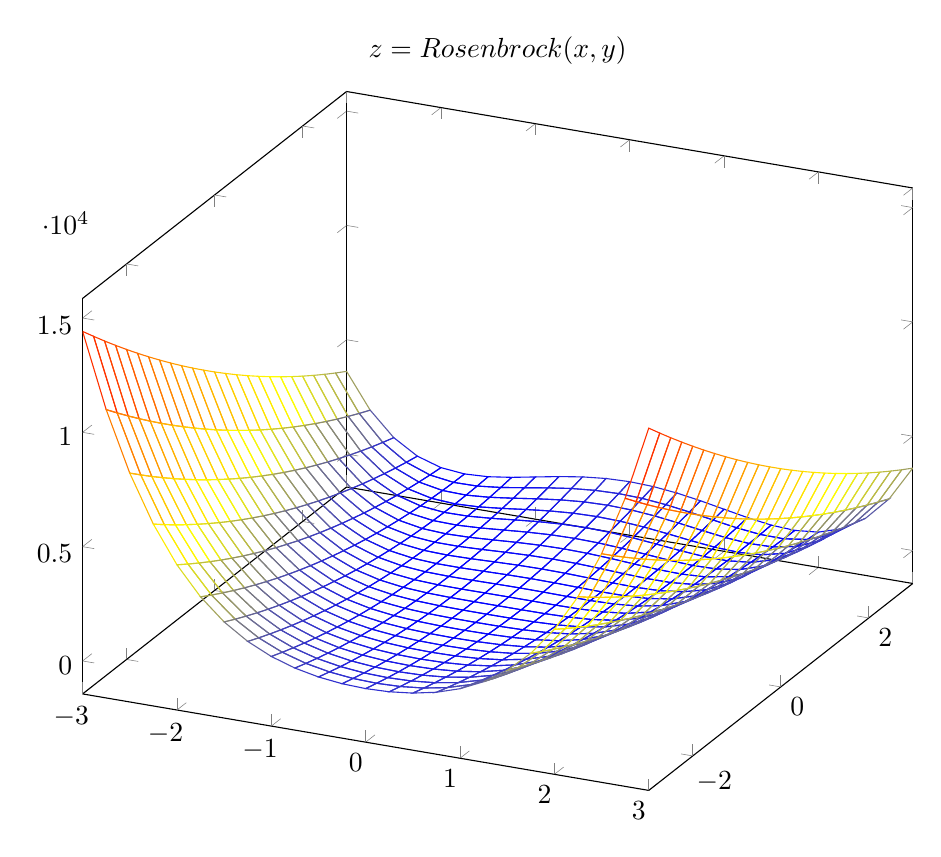
\begin{tikzpicture}
      \begin{axis}[width=\linewidth, title={$z=Rosenbrock(x, y)$}]
        \addplot3[mesh, domain=-3:3]{(1 - x)^2 + 100 * (y - x^2)^2};
      \end{axis}
    \end{tikzpicture}
  \end{subfigure}
  \begin{subfigure}[t]{0.3\linewidth}
    \center
    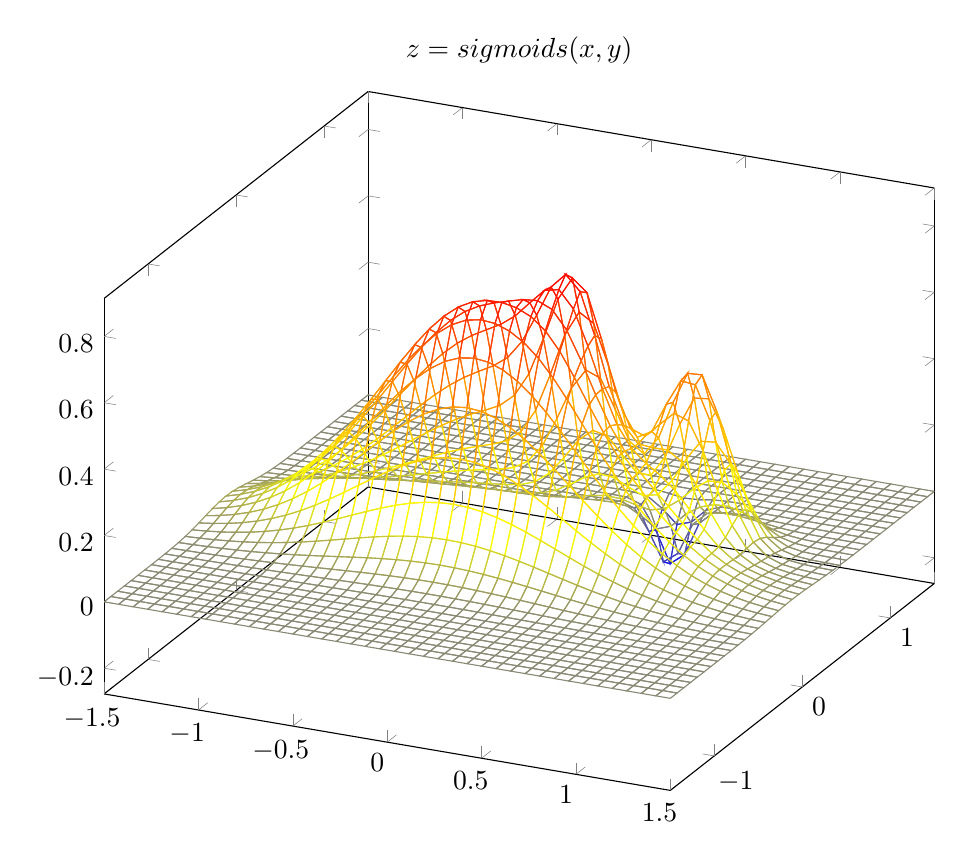
\begin{tikzpicture}
      \begin{axis}[width=\linewidth, title={$z=sigmoids(x, y)$}]
        \addplot3[mesh, samples=40, domain=-1.5:1.5]{0.5 * e^(- (((9*x-2)^2) + ((9*y-2)^2)) / 4) + 0.75 * e^(- ((9*x+1)^2) / 49 - ((9*y+1)^2) / 10) + 0.5 * e^(- (((9*x-7)^2) + (9*y-3)^2) / 4) -0.2 * e^(-  ((9*x-4)^2) - (9*y-7)^2)};
      \end{axis}
    \end{tikzpicture}
  \end{subfigure}
  \caption{Тестовые модели}
  \label{img:functionz}
\end{figure}



%--------------------------------------------------------------------


\subsection{Схемы кодирования дерева}

\subsubsection{Префиксное кодирование}

В исходном алгоритме ПЭГ декодирование дерева производится путём линейного извлечения элементов генома и установки в узлы формируемого дерева при его обходе в ширину. При замене обхода дерева в ширину обходом в глубину повышается связность генома~--- уменьшается расстояние между элементами, соответствующими соседним узлам дерева, а под-дерево кодируется непрерывной строкой в геноме. Такой подход способствует сохранению субструктур, что делает менее разрушительным применение операторов скрещивания~\cite{Li:gecco05lbp}. Сохранение в популяции субструктур (суб-деревьев) лучших особей и их рекомбинация позволяет ускорить сходимость алгоритма: оптимальное решение обнаруживается на более ранних поколениях (в несколько раз быстрее), качество оптимального решения зачастую выше, чем результат работы оригинального алгоритма ПЭГ.

Однако при таком подходе разрушается гарантия получения синтаксически корректного дерева из любого генома, сформированного согласно правилам. Потому требуется ввести процедуру динамической валидации дерева. К участию в эволюционном процессе допускаются только те особи, декодирование которых порождает корректное дерево. Такая система получила название P-GEP.

От предыдущих авторов. Предложенная линейная структура генома делает возможнным легко выделять из него отдельные под-деревья, что, в свою очередь, позволяет производить поиск повторяющихся субструктур. Появление часто встречающихся субструктур в лучших особях популяции означает их высокую полезность при составлении конечного решения. Выделив набор таких субструктур популяции авторами предлагается формировать из них т.н. элитную группу~\cite{Substructures(ICMLA05)_XLi}. Каждый элемент этой группы обозначается одним дополнительным терминальным символов.

Для взаимодействия между особями и элитной группой были введены два новых генетических оператора: оператор сжатия, заменяющий последовательность в геноме особи соответствующим терминальным символом из элитной группы, и оператор раскрытия, выполняющий обратную операцию~--- замену терминального символа на соответствующую последовательность из элитной группы.
Внесение данной модификации в P-GEP привело к обнаружению решений, имеющих значительно меньшую погрешность.

%--------------------------------------------------------------------

\subsubsection{Кодирование с наложениями}

В работе~\cite{conf/icnc/PengTZY05} рассматривается разновидность декодирования генома путём обхода дерева в глубину, при котором последовательно идущие под-деревья накладываются друг на друга. Элементы генома последовательно считываются:
\begin{itemize} \itemsep0pt \parskip0pt \parsep0pt
  \item Если текущий символ принадлежит к терминальному множеству~--- поместить его в синтаксическое дерево как листовой узел.
  \item Если текущий символ принадлежит к функциональному множеству~--- поместить его в синтаксическое дерево как узел с количеством дочерних узлов, равным количеству аргументов помещаемой функции. Первый дочерний узел~--- следующий в геноме за текущим, второй~--- следующий за ним и т.д. Дочерние под-деревья заполняются следуя этой же процедуре.
  \item При выходе за пределы генома в качестве текущего символа берётся первый элемент терминального множества.
\end{itemize}

Коренное отличие описанного способа декодирования коренным образом отличается от методов обхода в ширину и обхода в глубину тем, что элементы генома могут быть задействованы в построении дерева неоднократно, и размер получаемого дерева, как правило, больше при равном размере генома.

Рассмотрим на примере строки <<\verb|**a+*bc|>>, синтаксическое дерево, образующееся при её декодировании, показано на рисунке~\ref{img:GEP_ET_sample_EAOGE}.

\begin{figure} [h]
  \center
  \begin{tikzpicture}[level distance=1cm,
    level 1/.style={sibling distance=3cm},
    level 2/.style={sibling distance=2cm},
    level 3/.style={sibling distance=1cm}]
    \tikzstyle{every node}=[-,thick]
    \node { $\times$ }
      child[->] { node { $\times$ }
        child { node { $a$ } }
        child { node { $+$ }
          child { node { $\times$ }
            child { node { $b$ } }
            child { node { $c$ } }
          }
          child { node { $b$ } }
        }
      }
      child[->] { node { $a$ } }
      ;
  \end{tikzpicture}
  \caption{Пример дерева, декодированного с наложениями}
  \label{img:GEP_ET_sample_EAOGE}
\end{figure}

При использовании традиционного метода декодирования, принятого в ПЭГ, данному дереву соответствует строка <<\verb|**aa+*bbc|>>, содержащая на 2 символа больше.

Выразительная сила генома при декодировании с наложениями значительно выше, что показано в таблице~\ref{tbl:EAOGE_expression_power}, отражающей соответствие максимального возможного размера (количества узлов) синтаксического дерева при равных размерах гена.

\begin{table}[h]
  \caption{Сравнение выразительной силы ПЭГ с наложениями}
  \label{tbl:EAOGE_expression_power}
  \begin{center}
    \begin{tabular}{|c|c|c|}
      \hline
      Размер гена & ПЭГ & ПЭГ с наложениями \\
      \hline
      3 & 3 & 9 \\
      5 & 5 & 25 \\
      7 & 7 & 67 \\
      9 & 9 & 177 \\
      11 & 11 & 465 \\
      13 & 13 & 1219 \\
      15 & 15 & 3193 \\
      17 & 17 & 8361 \\
      \hline
    \end{tabular}
  \end{center}
\end{table}

Повышение выразительной силы генома позволяет использовать более короткие хромосомы, что, в свою очередь, значительно понижает вычислительную сложность алгоритма: разница в скорости обработки экспоненциально растёт, при длине хромосомы в 23~элемента ускорение достигает 10~раз. Авторы подхода назвали систему на его основе EAOGE~--- Evolutionary Algorithm based on Overlapped Gene expression~--- эволюционный алгоритм на осове ПЭГ с наложениями. 

Сравнение эффективности реализованной системы ПЭГ с данной модификацией, исходным алгоритмом и ПЭГ с префиксным кодированием приведено в таблице~\ref{tbl:cmp_tree_depths}, для возможности сопоставления производительности алгоритмов было зафиксировано время, выделяемое каждому запуску.

При небольшой длине генома ПЭГ с наложениями существенно превосходит конкурирующие модификации в способности обнаруживать отличные решения. Дальнейшее увеличение максимально возможного размера дерева до глубины в 4~узла несколько меняет картину: префиксное ПЭГ значительно выигрывает в вероятности успешного обнаружения решения, в то время как выходом ПЭГ с наложениями является лучшая модель. При допущении деревьев глубиной в 5~узлов наилучшее показатели имеет префиксное ПЭГ, показатели всех алгоритмов достигают своего максимума.

Таким образом, обе модификации превосходят исходный алгоритм в производительности, однако каждая из них занимает свою нишу, потому выбор одной из них определяется в зависимости от нужд исследователя.

\input{cmp_tree_depths}

%--------------------------------------------------------------------

\subsubsection{Нейтральные гены}

После декодирования хромосомы ПЭГ и конструирования синтаксического дерева количество узлов полученного дерева в предельном случае будет равно размеру хромосомы, однако в большинстве случаев будет меньшим. Те элементы в хвостах генов, которые не были использованы при построении дерева, называются некодирующими участками. Кроме того, полученное дерево может содержать выражения вида $(a - a)$, $(a \times 0)$, $(a - 0)$ и т.п., которые при семантическом анализе упрощаются, устраняя данные интроны и образуя более компактное дерево. Множество подобных участков~--- часто повторяющихся последовательностей, интронов, псевдогенов и пр.~--- встречается в природе в ДНК живых существ. Потому логично предположить, что и в искусственном геноме нейтральные участки могут быть полезны. Среднее количество нейтральных последовательностей в популяции растёт с увеличением как количества генов в хромосоме, так и размера каждого из них.

Исследования работы алгоритма с различной длиной генома показали~\cite{journals/advcs/Ferreira02}, что эволюционирование особей с высокой степенью избыточности генома происходит эффективней. Это связано с тем, у каждого решения, представленного в наиболее компактной форме, существует множество менее компактных вариантов представления, увеличенных в размерах за счёт интронов. Кроме того, накапливаемые в некодирующих участках мутации могут быть задействованы в дальнейшем, если изменения в голове гена (добавление функциональных узлов) приведут к увеличению размера дерева. В таблице~\ref{tbl:cmp_tree_depths} приведены результаты моделированя с различной длиной генома. Удлиннение генома ведёт к возрастанию пространства поиска, появлению деревьев б\'{о}льшего размера, следовательно, ведёт к более длительному расчёту популяции. Имеет смысл сравнивать модели, на построение которых было затрачено равное время. В приведённой таблице видно, что для каждой задачи имеется некая оптимальная длина генома. Меньший размер генов не позволяет выразить деревья достаточной сложности, а при б\'{о}льшем требуется на порядки больше вычислительного времени.



%--------------------------------------------------------------------



\subsection{Создание начальной популяции}

В изученных работах, посвящённых ПЭГ, не уделяется внимания процедуре создания начальной популяции, а именно конструированию случайной особи. Указывается, что строка хромосомы обходится с начала и по порядку, и каждый символ задаётся случайным образом: тип узла может быть равновероятно задан как функциональный элемент, как переменная (подаваемая на вход модели) и как числовая константа. Очевидно, что размер дерева определяется количеством подряд (близко) идущих функциональных узлов, начиная с корневого узла (первого символа хромосомы): из условия равновероятности типов узлов (3 типа~--- 33.333\%~каждый) следует, что вероятность создания дерева, состоящего всего из одного элемента (терминала: переменной либо константы), составляет~66.67\%. При этом можно заметить, что средняя длина получаемых деревьев не зависит от задаваемой длины хромосомы, но определяется установленной вероятностью появления того или иного типа.

При оригинальном кодировании элементов путём обхода узлов дерева в ширину логично предположить, что вероятность появления функциональных узлов в головной части хромосомы следует повысить, в то время как в хвостовой части могут быть помещены исключительно терминальные узлы. В таком случае определение оптимальных численных значений вероятностей представляет собой отдельную задачу для исследования. Кроме того, данный подход не применим к другим способам кодирования, потому не обладает должной универсальностью.

Для решения указанной проблемы и закрепления взаимосвязи между размером дерева и длиной генома была разработана следующая процедура инициализации. Обход строки так же производится посимвольно, начиная с её начала (независимо от способа кодирования). При этом не составляет трудности определить местонахождение кодируемого символом узла в дереве, а именно его глубину: первый символ является корневым узлом, далее~--- в соответствии со способом кодирования.

Вырожденное дерево, состоящее из одного терминала, как правило, не представляет интереса, так как решаемая таким образом задача не требует применения ПЭГ. В таком случае вероятность задания функционального типа корневому узлу устанавливается равным~100\%. В тоже время для ограничения размера дерева заданным значением (несмотря на способность префиксного кодирования и ПЭГ с наложениями создания деревьев, превышающих в размере длину генома) в целях удобства пользования уместно ограничить узлы максимальной возможной глубины листовыми. Следовательно, вероятность появления функционала в указанных местах равна нулю. Требует решения задача распределения вероятности функциональных узлов в зависимости от глубины вложенности.

Предлагается использование следующей формулы:

\begin{equation}
\label{eq:init_func_prob}
P_{func}(level, maxlevel) = \sqrt{1 - \left(\frac{level - 1}{maxlevel - 1}\right)^2}
\end{equation}

где $level$~--- глубина узла, $maxlevel$~--- максимально возможная глубина дерева. Пример такого распределения показан на рисунке~\ref{img:init_func_prob}.

\begin{figure} [h]
  \center
  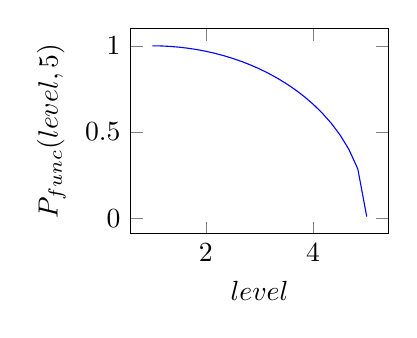
\begin{tikzpicture}[domain=1:5]
  	\begin{axis}[xlabel={$level$}, ylabel={$P_{func}(level, 5)$}, width=0.4\linewidth, no marks]
      \addplot{sqrt(1 - ((x - 1) / (5 - 1))^2)};
    \end{axis}
  \end{tikzpicture}
  \caption{Вероятность появления функционального узла в зависимости от глубины узла в дереве глубиной 5}
  \label{img:init_func_prob}
\end{figure}

Таким образом, процедура инициализации задает узлу глубины~$level$ тип функции при выполнении условия $random(0\ldots1) < P_{func}(level, maxlevel)$, обеспечивая сбалансированную начальную популяцию особей прогнозируемого размера. Данный метод конструирования новой особи случайным образом показал свою эффективность и был использован во всех экспериментах.



%--------------------------------------------------------------------


\subsection{Выводы}

В данной статье был проанализирован алгоритм ПЭГ, рассмотрены различные схемы кодирования синтаксических деревьев для их последующей линеаризации и хранения, описана детальная процедура создания начальной популяции, которой не было уделено внимания в изученных работах. Была разработана универсальная методика, позволяющая определить производительность модификаций алгоритма по любым метрикам, две из которых были отобраны как представляющие наибольший интерес. Сравнение схем кодирования выявило их эффективное применение.

